% !TeX spellcheck = en_GB
\documentclass[aspectratio=169]{beamer}
\usepackage{fontspec}
\usepackage[T1]{fontenc}
\usepackage{amsmath}
\usepackage{amsfonts}
\usepackage{amssymb}
\usepackage{graphicx}
\usepackage{csquotes}
\usepackage{booktabs}
\usepackage{multicol}
\usepackage{enumerate}
\usepackage{microtype}
\usepackage[labelfont=bf,font={small}]{caption}
\usepackage{hyperref}
\usepackage{booktabs}
\usepackage{subcaption}
\usepackage{fancyhdr}
\usepackage{pdfpages}
\usepackage{siunitx}
\usepackage{tikz}
\usepackage{mdframed}

\defaultfontfeatures{Mapping=tex-text}
\newfontfamily\symbolfont{Symbola}
\newfontfamily\quotefont{Gentium}

\usepackage[sorting=none]{biblatex}
\addbibresource{../bibliography.bib}

\author{Andreas Stöckel}


\renewcommand{\vec}[1]{{\mathbf{#1}}}
\newcommand{\mat}[1]{{\mathbf{#1}}}
\newcommand{\T}{\ensuremath{\mathsf{T}}}
\renewcommand{\epsilon}{\varepsilon}
\renewcommand{\phi}{\varphi}

% Tango color palette
\definecolor{butter1}{HTML}{FCE94F}
\definecolor{butter2}{HTML}{EDD400}
\definecolor{butter3}{HTML}{C4A000}
\definecolor{orange1}{HTML}{FCAF3E}
\definecolor{orange2}{HTML}{F57900}
\definecolor{orange3}{HTML}{CE5C00}
\definecolor{chocolate1}{HTML}{E9B96E}
\definecolor{chocolate2}{HTML}{C17D11}
\definecolor{chocolate3}{HTML}{8F5902}
\definecolor{chameleon1}{HTML}{8AE234}
\definecolor{chameleon2}{HTML}{73D216}
\definecolor{chameleon3}{HTML}{4E9A06}
\definecolor{skyblue1}{HTML}{729FCF}
\definecolor{skyblue2}{HTML}{3465A4}
\definecolor{skyblue3}{HTML}{204A87}
\definecolor{plum1}{HTML}{AD7FA8}
\definecolor{plum2}{HTML}{75507B}
\definecolor{plum3}{HTML}{5C3566}
\definecolor{scarletred1}{HTML}{EF2929}
\definecolor{scarletred2}{HTML}{CC0000}
\definecolor{scarletred3}{HTML}{A40000}
\definecolor{aluminium1}{HTML}{EEEEEC}
\definecolor{aluminium2}{HTML}{D3D7CF}
\definecolor{aluminium3}{HTML}{BABDB6}
\definecolor{aluminium4}{HTML}{888A85}
\definecolor{aluminium5}{HTML}{555753}
\definecolor{aluminium6}{HTML}{2E3436}

\definecolor{violet}{HTML}{AA305C}
\definecolor{uwyellow}{HTML}{FDD433}
\definecolor{background}{HTML}{F9F9F6}
\definecolor{text}{HTML}{000000}

\definecolor{uweng1}{HTML}{D1B2EE}
\definecolor{uweng2}{HTML}{BF33DE}
\definecolor{uweng3}{HTML}{8001B3}
\definecolor{uweng4}{HTML}{56048A}

\setbeamercolor{title}{fg=violet}
\setbeamercolor{frametitle}{fg=black}
\setbeamercolor{structure}{fg=aluminium5}
\setbeamercolor{normal text}{fg=text}

\setbeamertemplate{navigation symbols}{}
\setbeamertemplate{footline}[frame number]

\hypersetup{%
	colorlinks=false,% hyperlinks will be black
	urlbordercolor=aluminium4,% hyperlink borders will be red
	pdfborderstyle={/S/U/W 0.5}% border style will be underline of width 1pt
}

\makeatletter
\newcommand{\superimpose}[2]{%
	{\ooalign{{#1}\hidewidth\cr{#2}\hidewidth\cr}}}
\makeatother
\newcommand{\SolidCircle}[2]{\superimpose{\color{#1}\symbolfont ⬤}{\textbf{\color{white}#2}}\hspace{1em}}
\newcommand{\OPlus}{\SolidCircle{chameleon3}{\kern0.75pt+}}
\newcommand{\OMeh}{\SolidCircle{uwyellow}{~}}
\newcommand{\OMinus}{\SolidCircle{scarletred3}{\kern2.25pt--}}

\newcommand{\hl}[1]{\colorbox{uwyellow}{{\color{black}\textbf{#1}}}}

\newcommand{\ImageSources}[1]{%
	\begin{columns}%
		\column{1.1\textwidth}%
		\raggedright%
		\tiny\color{aluminium4}%
		\setlength\lineskip{1em}%
		\textbf{Image Sources.}	{#1}%
	\end{columns}}

\newcommand{\ColorRect}[3]{{\color{#1}\rule{#2}{#3}}}
\setbeamertemplate{headline}{\ColorRect{black}{\textwidth}{4pt}\newline\ColorRect{uweng1}{0.25\textwidth}{4pt}\ColorRect{uweng2}{0.25\textwidth}{4pt}\ColorRect{uweng3}{0.25\textwidth}{4pt}\ColorRect{uweng4}{0.25\textwidth}{4pt}}

\newcommand{\MakeTitle}{%
	\vspace{0.5cm}%
	{\textbf{\inserttitle}}\\[0.5cm]%
	\insertauthor\\[0.5cm]%
	\insertdate\\%
	\vspace{2cm}%
 	
\includegraphics[width=7cm]{../assets/uwlogo_eng.pdf}%
}

\newcommand{\handwritingframe}{%
	\begin{frame}
		\begin{columns}
			\column{\paperwidth}
			
\includegraphics{../assets/handwriting_lines.pdf}
		\end{columns}
	\end{frame}	
}

\newcommand{\imageframe}[1]{%
	\setbeamertemplate{navigation symbols}{}%
	\begin{frame}[plain,noframenumbering]%
		\begin{tikzpicture}[remember picture,overlay]%
		\node[at=(current page.center)] {%
			\includegraphics[width=\paperwidth]{#1}%
		};%
		\end{tikzpicture}%
	\end{frame}%
}

\newcommand{\videoframe}[3][mp4]{%
	\begin{frame}[plain,noframenumbering]%
		\hypersetup{%
			pdfborderstyle={/S/U/W 0}% border style will be underline of width 1pt
		}%
		\begin{tikzpicture}[remember picture,overlay]%
		\node[at=(current page.center)] {%
			\includegraphics[width=\paperwidth]{{{video/#2_#3}.jpg}}%
		};%
		\node[at=(current page.center)] {%
			\ifcsname SlidesDistr\endcsname%
				\href{https://youtu.be/#3}{
\includegraphics[width=2cm]{../assets/play_button.pdf}}%
			\else%
				\href{video/#2_#3.#1}{
\includegraphics[width=2cm]{../assets/play_button.pdf}}%
			\fi%
		};%
		\end{tikzpicture}%
	\end{frame}%
}

\newcommand{\includevideo}[4][mp4]{%
	\begingroup%
	\hypersetup{%
		pdfborderstyle={/S/U/W 0}% border style will be underline of width 1pt
	}%
	\begin{tikzpicture}%
	\node (A) {%
		\includegraphics[width=#4]{{{video/#2_#3}.jpg}}%
	};%
	\node[at=(A.center)] {%
		\ifcsname SlidesDistr\endcsname%
			\href{https://youtu.be/#3}{
\includegraphics[width=2cm]{../assets/play_button.pdf}}%
		\else%
			\href{video/#2_#3.#1}{
\includegraphics[width=2cm]{../assets/play_button.pdf}}%
		\fi%
	};%
	\end{tikzpicture}%
	\endgroup%
}

\newcommand{\backupbegin}{
	\newcounter{finalframe}
	\setcounter{finalframe}{\value{framenumber}}
	\setbeamertemplate{footline}{}
}

\newcommand{\backupend}{
	\setcounter{framenumber}{\value{finalframe}}
}


\date{September 8, 2021}
\title{SYDE 556/750 \\ Simulating Neurobiological Systems \\ Lecture 0: Administrative Remarks}

\begin{document}
	
\begin{frame}{}
	\MakeTitle
\end{frame}

\begin{frame}{Organization (I)}
	\begin{block}{Instructor}
		\vspace{2mm}
		\textbf{Terry Stewart}\\[2mm]
		\hspace{-2.5mm}\begin{tabular}{l l}
			Email & \url{terry.stewart@gmail.com}\\
			Website & \url{https://terrystewart.ca}\\
		\end{tabular}
	\end{block}
 
	\vfill

	\begin{block}{Course website}
		\begin{itemize}
			\item \url{https://github.com/tcstewar/syde556-f21}
			\item \url{syde556-f21.slack.com}
		\end{itemize}
	\end{block}
\end{frame}

\begin{frame}{Organization (II)}
	\begin{block}{Course times and logistics}
		\begin{itemize}
			\item \textbf{Saturday:}\\
			Pre-recorded lectures posted
			\item \textbf{Monday:}\\
			8:30-9:50 online lecture and discussion (LEARN)
			\item \textbf{Tuesday:}\\9:00-9:50 online discussion (LEARN) (SYDE 750, optional for 556)
			\item \textbf{Wednesday:}\\
			8:30-9:50 online lecture and discussion (LEARN) 
			\item \textbf{Any time:}\\
Email \url{terry.stewart@gmail.com}\\ Slack \url{syde556750-f21.slack.com} 
		\end{itemize}
	\end{block}

\end{frame}

\begin{frame}{Textbooks and Readings}
	\begin{columns}[T]
		\column{0.2\textwidth}
			\raggedleft
			\fboxrule=0.4pt\fboxsep=0pt\fbox{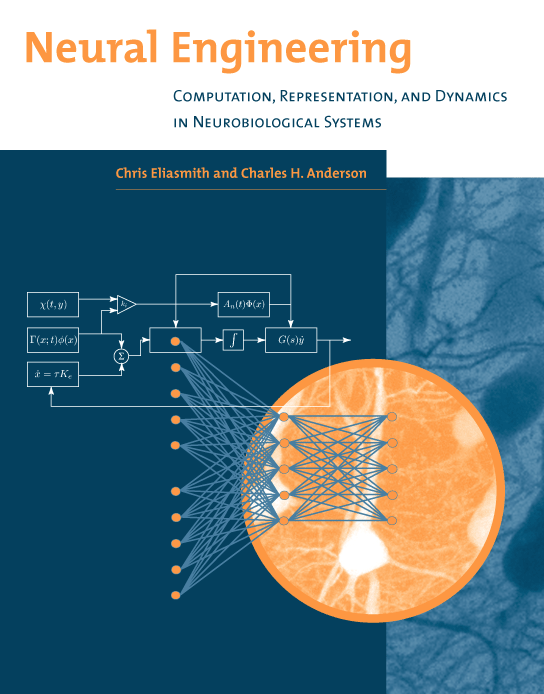
\includegraphics[height={\dimexpr 0.4\textheight - 0.8pt}]{media/neural_engineering_cover.png}}\\
		\column{0.3\textwidth}  
			\small
			\textbf{Main text:}\\
			Chris Eliasmith and\\Charles H. Anderson\\
			\emph{Neural Engineering: Computation, Representation, and Dynamics in Neurobiological Systems}, MIT Press, 2003.
		\column{0.2\textwidth}
			\raggedleft
			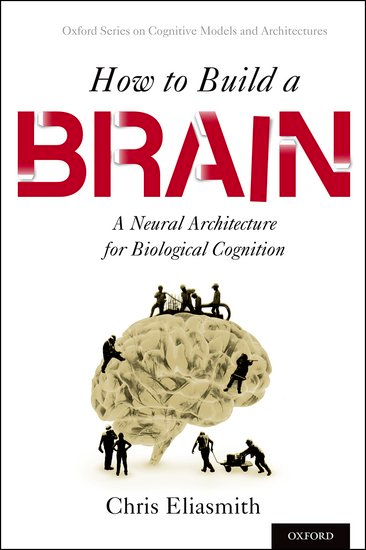
\includegraphics[height=0.4\textheight]{media/how_to_build_a_brain_cover.png}\\
		\column{0.3\textwidth}
			\small
			\textbf{Optional:}\\
			Chris Eliasmith\\
			\emph{How to Build a Brain}, Oxford University Press, 2013.
	\end{columns}
\end{frame}

\begin{frame}{Coursework (SYDE 556 \& SYDE 750)}
	\begin{columns}[t]
		\column{0.5\textwidth}
		\begin{block}{\hl{Five Assignments}}
		\begin{itemize}
				\item 20\%, 20\%, 15\%, 15\%, 30\%, respectively
				\item Roughly two weeks for each assignment
				\item Everyone must write their own code, generate their own graphs, and write their own answers.
			\end{itemize}
		\end{block}
		\column{0.5\textwidth}
		\begin{block}{\hl{Final Project} (SYDE 750 only)}
			\begin{itemize}
				\item Build a model of some neural system.
				\item Replicable science: report everything needed to recreate your model and analysis
				\item 25\% of grade (assignments are rescaled to 75\%)
				\item Have your project proposal approved via email by Oct 27
			\end{itemize}
		\end{block}
	\end{columns}
\end{frame}

\begin{frame}{Coursework (SYDE 750 only)}
	\begin{block}{Class Participation in the Seminar  (SYDE 750 only; optional for SYDE 556)}
	\begin{itemize}
		\item General discussion about Neuroscience, cognitive science, AI, etc.
		\item Special interest: replicable science and computational modelling
		\item SYDE 750 students must attend the seminar (Tuesday, 9:00-9:50).
		\item No marks for this part of the course.
	\end{itemize}
	\end{block}
\end{frame}

\begin{frame}{Schedule (I)}
\small
\begin{tabular}{p{2cm} p{2cm} p{5cm} p{3cm}}
	\toprule
	\textbf{Date} &	\textbf{Reading} &	\textbf{Topic} & \textbf{Assignments} \\
	\tiny WEEK 1 & & & \\
	Sept 8 &
	Chapter 1 &
	Introduction &
	\\[0.05cm]
	\tiny WEEK 2 & & & \\
	Sept 13 &
	Chapter 2 &
	Neurons &
	\\
	Sept 15 &
	Chapter 2 &
	Population Representation (I) &
	\#1 posted
	\\[0.05cm]
	\tiny WEEK 3 & & & \\
	Sept 20 &
	Chapter 2 &
	Population Representation (II) &
	\\
	Sept 22 &
	Chapter 4 &
	Temporal Representation &
	\\[0.05cm]
	\tiny WEEK 4 & & & \\
	Sept 27 &
	 &
	Guest Lecture &
	\\
	Sept 29 & & Guest Lecture &
	\\[0.05cm]
	\tiny WEEK 5 & & & \\
	
	Oct 4 &
	Chapters 5, 6 &
	Feedforward Transformations (I) &
	\#1 due*, \#2 posted\\
	Oct 6 &
	Chapters 5, 6 &
	Feedforward Transformations (II) &
	\\[0.05cm]
	\tiny WEEK 6 & \multicolumn{3}{c}{\emph{--- Reading week, no lectures ---}} \\[0.05cm]
	
	\bottomrule
\end{tabular}
\end{frame}


\begin{frame}{Schedule (II)}
	\small
	\begin{tabular}{p{2cm} p{2cm} p{5cm} p{3cm}}
		\toprule
		\textbf{Date} &	\textbf{Reading} &	\textbf{Topic} & \textbf{Assignments} \\
		
		\tiny WEEK 7 & & & \\
		Oct 18 &
		Chapter 8 &
		Dynamics (I) &
		\\
		Oct 20 &
		Chapter 8 &
		Dynamics (II) &
		\\
		
		\tiny WEEK 8 & & & \\
		Oct 25 &
		Chapter 7 &
		Analysis of Representation &
		\#2 due*, \#3 posted\\
		Oct 27 &
		\emph{provided} &
		Temporal Basis Functions &
		\\
		&
		&
		&
		SYDE 750 Project proposal due\\[0.05cm]
		
		\tiny WEEK 9 & & & \\
		Nov 1 &
		\emph{provided} &
		Symbols (I) &
		\\
		Nov 3 &
		\emph{provided} &
		Symbols (II) &
		\\[0.05cm]
		
		\tiny WEEK 10 & & & \\
		Nov 8 &
		Chapter 8 &
		Memory &
		\#3 due*, \#4 posted\\
		Nov 10 &
		\emph{provided} &
		Action Selection &
		
		\\
		\bottomrule
	\end{tabular}
\end{frame}

\begin{frame}{Schedule (III)}
	\small
	\begin{tabular}{p{2cm} p{2cm} p{5cm} p{3cm}}
		\toprule
		\textbf{Date} &	\textbf{Reading} &	\textbf{Topic} & \textbf{Assignments} \\
		\tiny WEEK 11 & & & \\
		Nov 15 &
		Chaper 9 &
		Learning (I) &
		\\
		Nov 17 &
		Chaper 9 &
		Learning (II) &
		\\[0.05cm]
		\tiny WEEK 12 & & & \\
		Nov 22 &
		\emph{provided} &
		Spatial Semantic Pointers &
		\#4 due*\\
		Nov 24 &
		\emph{provided} &
		Biological Details &
		\\[0.05cm]
		
		\tiny WEEK 13 & & & \\
		Nov 29 &
		\emph{provided} &
		Other modelling frameworks &
		\\
		Dec 1 &
		&
		Conclusion &
		\\[0.05cm]
		
		\tiny WEEK 14 & & & \\
		Dec 6 &
		&
		Discussion &
		\\[0.05cm]
		
		\tiny WEEK 16 & & & \\
		Dec 23 &
		&
		&
		\#5 due; SYDE 750 projects due* \\
		\bottomrule
	\end{tabular}\\[0.2cm]
	\footnotesize
	* The project and all assignments are due at midnight ($\approx$ 11:59p Eastern) of that day.
\end{frame}

\begin{frame}{Homework}
	\begin{itemize}
		\setlength{\itemsep}{0.5cm}
		\item \textbf{Get the \hl{textbook}, read the first chapter}\\
		(\enquote{Neural Engineering}, Chris Eliasmith and Charles Anderson, 2003)
		\item \textbf{Be able to run \hl{\texttt{jupyter lab}} or (\texttt{jupyter notebook}) with \hl{Python 3}}\\
		Install \texttt{numpy}, \texttt{scipy}, and \texttt{matplotlib}. You may want to use \href{https://www.anaconda.com/distribution/}{Anaconda}, which ships with these packets preinstalled.
	\end{itemize}
\end{frame}

\end{document}